%%%%%%%%%%%%%%%%%%%%%%%%%%%%%%%%%%%%%%%%%%%%%%%%%%%%%%%%%%%%%%%%%%%%%%%%%%%%%%%%%%%%%%%%%%%%%%%%%%%%
\subsection{Fonctionnement global}
%%%%%%%%%%%%%%%%%%%%%%%%%%%%%%%%%%%%%%%%%%%%%%%%%%%%%%%%%%%%%%%%%%%%%%%%%%%%%%%%%%%%%%%%%%%%%%%%%%%%

Le fonctionnement global du projet sur la plateforme Androïd est relativement simple. Nous souhaitons
simplement pouvoir utiliser le téléphone portable comme un intermédiaire entre notre site web et le 
correspondant avec qui nous discutons. Pour cela le téléphone fait office de proxy entre les deux 
entités éloignées. Un proxy est un composant qui se place entre un interlocuteur et son auditeur. Le 
proxy sert principalement à relayer l'information d'un élément vers un autre, il sert d'intermédiaire.
Dans notre cas, le proxy s'occupe de recevoir des SMS et de les rediriger vers le site web. 
Réciproquement, il récupère les messages envoyés par le site web et envoie un SMS vers le correspondant
défini  dans le message reçu.



%%%%%%%%%%%%%%%%%%%%%%%%%%%%%%%%%%%%%%%%%%%%%%%%%%%%%%%%%%%%%%%%%%%%%%%%%%%%%%%%%%%%%%%%%%%%%%%%%%%%
\subsection{Création du service}
%%%%%%%%%%%%%%%%%%%%%%%%%%%%%%%%%%%%%%%%%%%%%%%%%%%%%%%%%%%%%%%%%%%%%%%%%%%%%%%%%%%%%%%%%%%%%%%%%%%%

Les applications fonctionnant sous Androïd régissent par un principe simple, celui des "activités".
Pour simplifier, une activité représente une fonctionnalité graphique d'une application. Par exemple,
lorsqu'une application est ouverte, on tombe sur un menu avec différentes possibilités d'actions 
qui nous sont offertes. Le menu représente donc ici une activité.
\\


Il faut savoir qu’une activité, lorsqu'elle est active, occupe le système qui attend des événements.
Si l'utilisateur ne fait rien alors que le menu est affiché, le système peut s'occuper d'autres 
tâches annexes. Si en revanche l'utilisateur navigue dans le menu, alors l'activité est considérée
comme en fonctionnement et bloque toutes autres opérations non relatives à l'application exécutée.
\\


Dans le cadre de notre application, nous devons à son lancement, effectuer une série d'opérations 
afin de mettre l'application en fonctionnement. Cela consiste notamment, à vérifier l'état de la 
connectivité internet, récupérer les identifiants et se connecter sur le service GTalk. Ces 
opérations rendent le système bloquant durant leur exécution. Cela n'est pas un problème lorsque la 
connection s'effectue sans erreur. Le traitement durant moins d'une seconde, le système n'est pas
gravement impacté. En revanche, si une erreur intervient, le programme va alors essayer de la résoudre.
Cela n'est pas concevable. En effet, une perte soudaine de réseau pourrait par exemple mettre 
l'application dans un état de recherche ce qui est potentiellement très lent. Cette situation rendrait
le terminal complètement bloqué durant la recherche. 

Ce comportement n'étant pas souhaitable, nous avons dû trouver une solution pour pouvoir outrepasser ce blocage.
\\


Nous avons alors utilisé le concept Androïd de "services". Celui-ci consiste à exécuter une fonctionnalité 
de manière asynchrone. Le service n'impacte pas le système, au contraire il fonctionne avec lui. 
 
\begin{figure}[!h]
  \center
  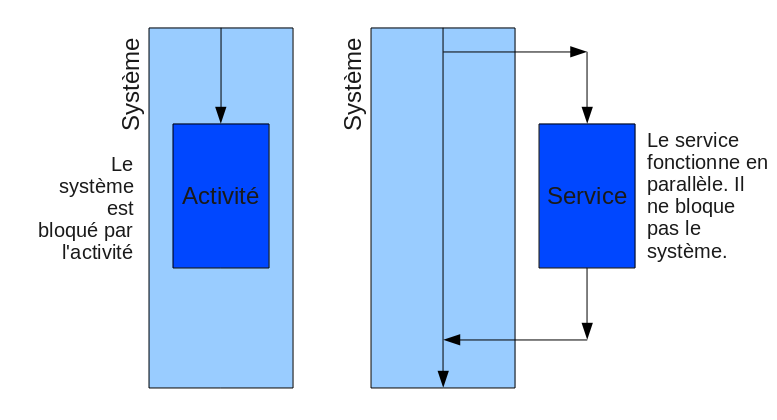
\includegraphics[width=13cm]{img/fonctionnement-des-services-android.png}
  \caption{Fonctionnement d'un service Androïd}
  \label{fonctionnement-des-services-android}
\end{figure}

Comme montré dans la figure \ref{fonctionnement-des-services-android}, le service n'est pas  bloquant. 
Lors de son exécution, le système continue de fonctionner sur d'autres tâches en paire avec le service lancé.
\\


Dans notre cas, le service sert à deux tâches principales. Tout d'abord il va configurer l'authentification
de l'utilisateur sur GTalk. Ensuite il va simplement se mettre en attente d'événements et le cas échéant, 
traiter ce même événement.



%%%%%%%%%%%%%%%%%%%%%%%%%%%%%%%%%%%%%%%%%%%%%%%%%%%%%%%%%%%%%%%%%%%%%%%%%%%%%%%%%%%%%%%%%%%%%%%%%%%%
\subsection{Authentification sur GTalk}
%%%%%%%%%%%%%%%%%%%%%%%%%%%%%%%%%%%%%%%%%%%%%%%%%%%%%%%%%%%%%%%%%%%%%%%%%%%%%%%%%%%%%%%%%%%%%%%%%%%%

Pour pouvoir converser avec le site web, l'application a besoin de s'authentifier auprès du service
GTalk. Pour cela, nous sommes passés par deux étapes. 
\\


Initialement, nous utilisions la méthode classique d'authentification. Lorsque l'utilisateur lance 
l'application, celle-ci lui demande de rentrer ses identifiant et mot de passe. Cela effectué, 
l'application se charge de se connecter et de s'authentifier sur les serveurs GTalk en utilisant les
paramètres rentrés par l'utilisateur.

Cette solution est la plus simple à implémenter mais n'est malheureusement pas la plus agréable
à utiliser ni la plus sure. Nous forçons en effet l'utilisateur à rentrer ses identifiants ce qui 
pourrait paraître légitime mais reste contraignant pour l'utilisateur. Celui-ci ne sait pas ce que 
nous faisons avec son mot de passe. Une application malveillante pourrait récupérer les identifiants
et s'en servir à des fins illégales. Dans notre cas, même si nous n'avions aucune mauvaise intention,
nous ne pouvons demander aux utilisateurs de nous faire confiance. Nous avons donc opté pour une 
deuxième solution, l'identification avec OAuth 2.0.
\\


Comme détaillé dans la partie \ref{Authentification avec OAuth 2.0}, OAuth permet de réaliser des actions en agissant à la place de l'utilisateur. 
Ici nous souhaitions simplement utiliser le compte GTalk de l'utilisateur sans que celui-ci ai à rentrer
ses identifiants. 

Contrairement à l'authentification sur le site web, l'authentification sur une plateforme Androïd est
théoriquement plus simple. En effet, une fois que l'utilisateur a donné son accord, le serveur 
d'authentification de Google va directement envoyer le token d'authentification. Il n'y a alors pas 
besoin d'effectuer une deuxième étape pour récupérer ce dernier comme le montre le diagramme 
\ref{obtention-token-avec-android}.

%%%%%%%%%%%%%%%%%%%%%%%%%%%%
%title Envoi d'un SMS
 
%Utilisateur->Application: délégation de l'authentification
%Application->Serveur Google: requête pour un token d'authentification
%Serveur Google->Application: token d'authentification
%Application->serveur GTalk: authentification(token)
%serveur GTalk->Application: authentification validé
%%%%%%%%%%%%%%%%%%%%%%%%%%%%

\begin{figure}[!h]
  \center
  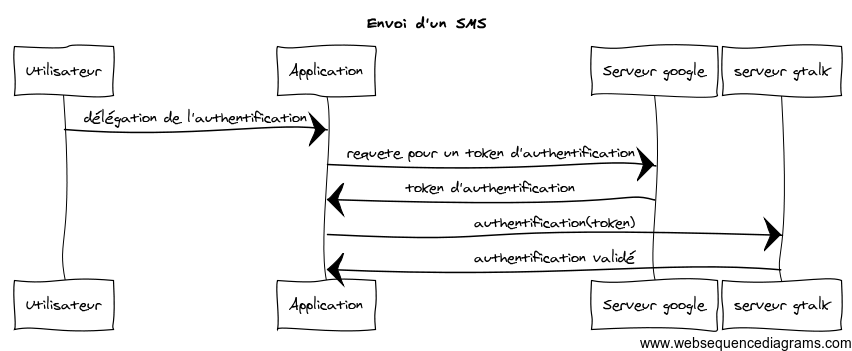
\includegraphics[width=15cm]{img/obtention-token-avec-android.png}
  \caption{Procédure d'obtention d'un token avec un appareil Androïd}
  \label{obtention-token-avec-android}
\end{figure}

% utilisation de aSmack ?
Néanmoins, une des difficultés d'implémenter ce protocole est que la librairie de gestion de compte
XMPP pour Androïd dénommée Asmack est différente de celle utiliser pour le site web. Asmack est un fork 
de la librairie Smack pour Androïd et est l'unique librairie gérant les comptes XMPP présente sur
Androïd. Ne souhaitant pas ré-implémenter toutes les fonctionnalités présentes dans celle-ci, nous avons
choisi de l'utiliser. Malheureusement, les différences entre les deux librairies nous ont empêché de 
ré-implémenter notre précédent travail effectué pour le site web qui était fonctionnel. 

Le langage Java fonctionne sur une machine virtuelle. Celle-ci contient des fonctionnalités basique sur
lesquelles le langage peut s'appuyer. Dalvik, la machine virtuelle pour Java présente sur Androïd n'est 
pas exactement la même que la machine virtuelle basique. En effet, pour des soucis de rapidité et de 
légèreté, certaines parties de Dalvik ont été réécrites pour en faire une machine virtuelle plus adaptée
aux plateformes mobiles.

Smack a été développé sur la machine virtuelle Java basique tandis que Asmack a été développé sur Dalvik.
Cette différence implique des changements quant aux fonctionnements de celles-ci.

Finalement, en ré-implémentant certaines fonctionnalités, nous avons réussi à nous authentifier avec OAuth.
\\


Authentifier un utilisateur via OAuth2.0 sur Androïd a été un réel challenge. Il nous a fallu comprendre 
et trouver des équivalences au fonctionnement de Smack.



%%%%%%%%%%%%%%%%%%%%%%%%%%%%%%%%%%%%%%%%%%%%%%%%%%%%%%%%%%%%%%%%%%%%%%%%%%%%%%%%%%%%%%%%%%%%%%%%%%%%
\subsection{Envoi et réception d'un SMS}
%%%%%%%%%%%%%%%%%%%%%%%%%%%%%%%%%%%%%%%%%%%%%%%%%%%%%%%%%%%%%%%%%%%%%%%%%%%%%%%%%%%%%%%%%%%%%%%%%%%%

\subsubsection{Réception d'un SMS}

Une fois authentifié, nous souhaitons pouvoir utiliser notre téléphone comme proxy. Notre application
doit en effet servir d'intermédiaire entre le site web et un correspondant. Pour cela elle doit tout
d'abord surveiller l'arrivée de nouveaux messages. 
\\


Google autorisent la surveillance du comportement du téléphone sur Androïd, permettant de réagir lors de différents événements.
Dans notre cas nous avons pu utiliser le principe de "Broadcast Receiver" du système. 
Un broadcast receiver est un outil qui permet de rendre une application consciente de son environnement.
Cela permet généralement à l'application qui l'utilise d'être prévenue lors de nouvelles notifications ou 
d'un comportement particulier du téléphone.
Son fonctionnement est simple : il permet de s'enregistrer auprès du téléphone qui maintient une base de donnée des membres à avertir lors d'un changement particulier.

\begin{figure}[!h]
  \center
  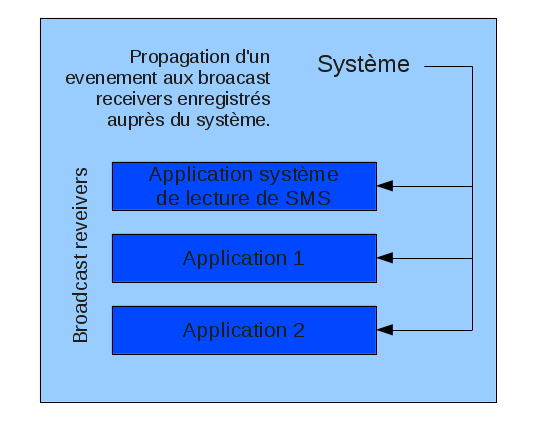
\includegraphics[width=12cm]{img/broadcast-receivers.png}
  \caption{Androïd : fonctionnement des broadcasts receivers}
  \label{broadcast-receivers}
\end{figure}

Le schéma \ref{broadcast-receivers} permet de voir le système du téléphone qui contient les différents broadcast receiver à avertir en cas de nouveaux messages. Ici l'application de rédaction de SMS ainsi que deux autres 
applications seront averties.

Dans notre cas, nous nous en sommes servis pour d'une part être avertis de l'arrivée de nouveaux SMS et d'autre part pour pouvoir récupérer le dit message et le traiter.


\subsubsection{Envoi d'un SMS}

L'envoi quant à lui est beaucoup plus trivial. Androïd met à disposition un outil permettant d'envoyer
des messages.

% développer ?



%%%%%%%%%%%%%%%%%%%%%%%%%%%%%%%%%%%%%%%%%%%%%%%%%%%%%%%%%%%%%%%%%%%%%%%%%%%%%%%%%%%%%%%%%%%%%%%%%%%%
%%%%%%%%%%%%%%%%%%%%%%%%%%%%%%%%%%%%%%%%%%%%%%%%%%%%%%%%%%%%%%%%%%%%%%%%%%%%%%%%%%%%%%%%%%%%%%%%%%%%
%%%%%%%%%%%%%%%%%%%%%%%%%%%%%%%%%%%%%%%%%%%%%%%%%%%%%%%%%%%%%%%%%%%%%%%%%%%%%%%%%%%%%%%%%%%%%%%%%%%%

\subsection{Fonctionnement}

%%%%%%%%%%%%%%%%%%%%%%%%%%%%%%%%%%%%%%%%%%%%%%%%%%%%%%%%%%%%%%%%%%%%%%%%%%%%%%%%%%%%%%%%%%%%%%%%%%%%

\subsubsection{Globalité}

Le fonctionnement global de notre application est relativement simple.
Elle a été tout d'abord implémentée de manière à répondre aux besoins du projet et être fonctionnelle pour donner une première version.

Lors de la réception d'un SMS sur le smartphone l'application va tout d'abord récupérer le contenu du message ainsi que son auteur.
Puis les données sont être encapsulée dans un message au format JSON.
Enfin le message est envoyé vers le webservice grâce à GTalk, qui s'occupera de notifier à l'utilisateur l'arrivée d'un nouveau message.

\begin{figure}[!h]
  \center
  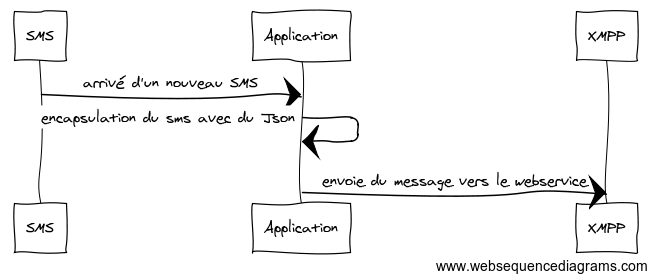
\includegraphics[width=12cm]{img/encapsulation-sms.png}
  \caption{Traitements lors de la réception d'un SMS}
  \label{encapsulation-sms}
\end{figure}

Lors de la réception d'un nouveau message XMPP la méthode est l'inverse de celle de la réception d'un SMS.
L'application va dé désencapsuler le message XMPP pour y récupérer l'information utile.
Cela fait, notre application va ensuite envoyer le SMS au destinataire.

%%%%%%%%%%%%%%%%%%%%%%%%%%%%%%%%%%%%%%%%%%%%%%%%%%%%%%%%%%%%%%%%%%%%%%%%%%%%%%%%%%%%%%%%%%%%%%%%%%%%

\subsubsection{Architecture}

Dans le cadre de notre projet, nous n'avions comme but, l'envoi de SMS à partir du webservice seulement.
Lors de la réception d'un message XMPP, nous souhaitions pouvoir réagir différemment en fonction du contenu du message.
Notre travail respectait donc ce principe mais ne permettait aucune évolutivité.

A supposer qu'un tiers soit intéressé par la communication entre le webservice et le téléphone par 
l'intermédiaire de XMPP, mais que son but ne soit pas d'envoyer de simple SMS, nous avons implémenté une
architecture permettant de rajouter facilement de nouvelles fonctionnalités. Pour donner des exemples, 
un utilisateur pourrait décider d'implémenter une fonctionnalité lui permettant de déclencher la capture
de photos de son téléphone à partir du webserver.
 
Pour permettre cette évolutivité, nous avons réalisé une architecture qui s'adapte automatiquement en
fonction des messages reçus. Il s'agit ici des patrons de conceptions fabrique et stratégie. 


\Jparagraph{Pattern stratégie}

Le patron de stratégie est un patron de conception de type comportemental.
Il permet d'adopter dynamiquement un comportement particulier en fonction des conditions de son exécution.
Concrètement, quelque soit la classe implémentant l'interface de base, l'exécution d'un algorithme s'effectue simplement depuis une seule méthode.
Le schéma \ref{pattern_strategie} décrit le fonctionnement du modèle.

\begin{figure}[H]
  \center
  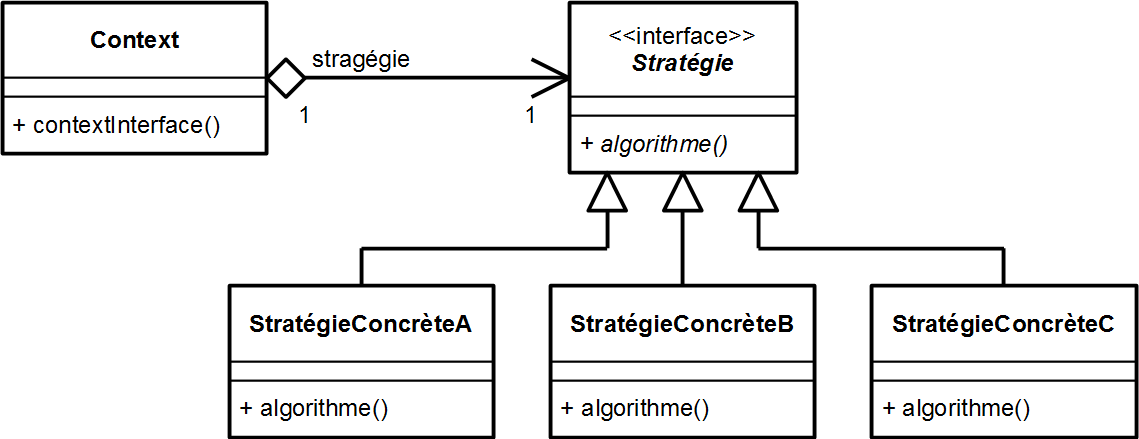
\includegraphics[width=12cm]{img/pattern_strategie.png}
  \caption{Pattern stratégie : diagramme UML}
  \label{pattern_strategie}
\end{figure}

Dans notre cas, il permet de créer différents types de stratégies qui pourront potentiellement être utilisés.
Notre projet ne contient pour l'instant que les stratégies "envoi de SMS" et "envoi de messages XMPP", mais avec cette architecture il est possible de rajouter d'autres stratégies, comme par exemple l'extinction du téléphone ou encore l'envoi d'un email par exemple.
\\


\Jparagraph{Pattern fabrique}

L'avantage du pattern stratégie est qu'il permet de regrouper les algorithmes à exécuter dans des classes séparées plutôt que de le mélanger dans du code différent.
Mais son inconvénient réside dans le fait qu'il est nécessaire d'effectuer un test sur le type d'algorithme à exécuter à chaque endroit où l'on doit instancier les stratégies.

Le pattern fabrique permet de palier à ce problème en définissant les règles d'instanciation des différentes stratégies.
Ainsi les différents tests ne se retrouvent pas dupliqués à chaque parties du code, mais regroupé dans une classe qui se chargera de définir la stratégie à appliquer en fonction des données qu'on lui transmet.
Le schéma \ref{pattern_fabrique} représente le diagramme de classe du pattern fabrique.
 
\begin{figure}[H]
  \center
  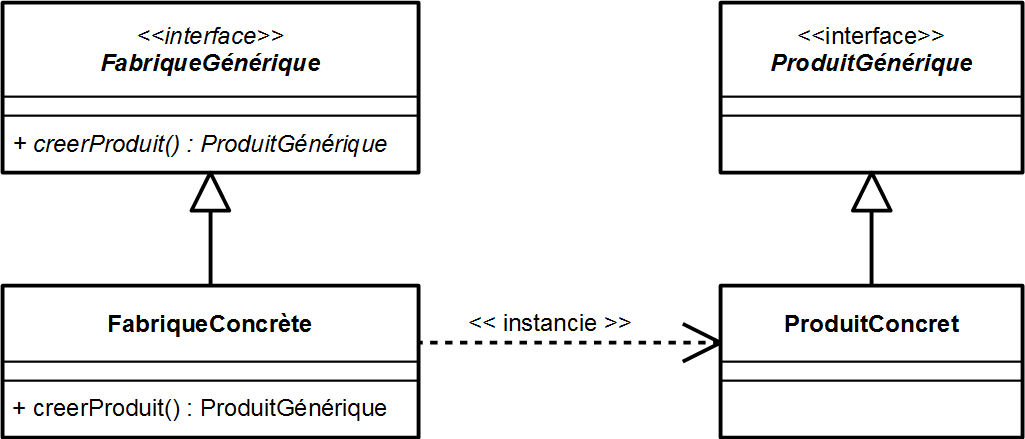
\includegraphics[width=10cm]{img/pattern_fabrique.png}
  \caption{Pattern fabrique : diagramme UML}
  \label{pattern_fabrique}
\end{figure}
 
Dans notre cas la fabrique va analyser chaque nouveau message.
En fonction de leurs contenus elle devra décider d'une stratégie.
\\


\Jparagraph{Ajout de fonctionnalités}

\begin{figure}[!h]
  \center
  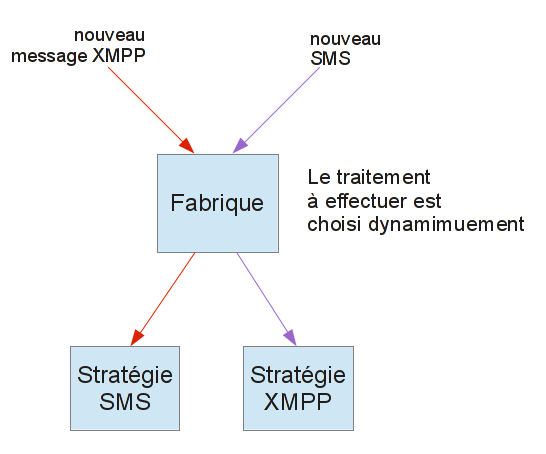
\includegraphics[width=10cm]{img/fonctionnement-strategie-factorie.png}
  \caption{Pattern fabrique : fonctionnement}
  \label{fonctionnement-strategie-factorie}
\end{figure}

La figure \ref{fonctionnement-strategie-factorie} montre le fonctionnement du projet lors de l'arrivée d'un
nouveau message (SMS ou XMPP).
L'intérêt principal de ce pattern est l'évolutivité qu'il apporte.
Le choix dynamique à l'exécution de la stratégie à un intérêt pour le développeur.
En effet, celui-ci n'a plus besoin de se soucier de l'implémentation du choix de la stratégie ni de son exécution.

L'ajout d'une fonctionnalité ne se fait plus dans chaque partie du code source, mais en définissant une nouvelle stratégie (classe représentative) puis en ajoutant sa définition dans la fabrique.
